\documentclass[11pt]{article}
\usepackage{cs65f12}
\usepackage{times}
\usepackage{latexsym}
\usepackage{ulem}
\usepackage{graphicx}
\setlength\titlebox{6.5cm}    % Expanding the titlebox

\title{BatTrace: Android battery performance testing via system call tracing}

\author{Yeayeun Park\\
{\tt ypark2@swarthmore.edu}
\And 
Mark Serrano\\
{\tt mserran2@swarthmore.edu}
\AND
Craig Pentrack\\                 
{\tt cpentra1@swarthmore.edu}}

\date{10/04/13}

\begin{document}
\maketitle
\begin{abstract}
  The increasing number of tasks we can perform on our mobile devices 
  feeds positively into the demand for devices with longer battery power. 
  Since mobile devices have become integral parts of our daily lives with
  the number of task we can accomplish far outpacing battery performance 
  improvements, consumers have increasingly encountered the issue of 
  efficient device usage and batter life management. In this paper, we 
  examine Android devices in particular and present BatTrace, an Android 
  analysis platform that evaluates battery performance on the android platform
  by tracing system calls. BatTrace will execute different types of popular system
  calls, and extract the correlation between a particular system call and its 
  influence on the battery. Subsequently, it will trace system calls made by 
  individual Android applications and use system call performance data to profile
  each application. Finally, the analysis on the correlation between system calls and their 
  battery usage, as well as the correlation between each application and system 
  calls they initiate, will be combined to produce the estimated battery performance 
  of on individual Android applications.
\end{abstract}

\section{Motivation}

Our project is motivated by an issue that we face daily: limited battery power 
on our mobile devices. The vast power available at our fingertips in mobile
devices is tamed by the amount of battery physically available. Given 
that dynamic analysis executes data in real-time to evaluate and test programs, 
we searched for tools that would allow us to perform dynamic analysis on our 
mobile devices while uncovering low-level explanations as to what is really 
draining the battery. By profiling particular system calls in terms of their battery
usage, we're hoping to derive a correlation between the two. Subsequently, with the
appropriate tools (such as 'strace') we plan to trace system calls made by third 
party applications and, in turn, provide a good set of guidelines for mobile users 
to follow, when the low battery crisis hits.

\section{Background}

Historically much power consumption research has focused on using utilization-based
methods.  However, modern smartphones employ complex power strategies in device 
drivers and OS-level power management, sometimes rendering utilization as a poor 
model for representing power states and deducing battery usage ~\cite{pathak-systemcall}.  While 
sometimes strong correlation exists between utilization and power consumption, often 
applications have constant power consumption while in certain states (while 
utilization fluctuates) or have high power consumption while low utilization ~\cite{pathak-systemcall,google-androiddev}.  
Additionally, measuring utilization via performance counters results in accuracy 
loss ~\cite{pathak-systemcall}.  Instead of modeling power with utilization, system calls, the only way of 
interacting with hardware and performing I/O, serve as a much more precise indicator 
of power consumption ~\cite{pathak-systemcall}.  Past work and tools, such as eProf, have shown systems 
calls to be an effective way of modeling power ~\cite{pathak-systemcall,yoon-appscope,pathak-eprof,ding-signals}.  Using the findings 
of eProf and other studies as justification, we plan to measure and classify system 
calls on Android smartphones in terms of their effect on battery life.

While eProf foregrounded system calls as an effective indicator of changes in power
state, eProf used systems calls as means to profiling applications with regard to power 
consumption on a sub-routine level ~\cite{pathak-systemcall,pathak-eprof}.  Developing models based off of system 
calls supplied a powerful tool, however the eProf research did not study battery drain 
as a result of  particular system calls themselves and the frequency with which 
applications rely on certain system calls.  Other work in the smartphone battery life 
research, including detecting energy-related bugs, correlating wireless signal strength 
with battery consumption, and generating battery usage information on the process or 
application level, has relied on system calls ~\cite{yoon-appscope,pathak-bugs,ding-signals}.  We plan to supplement the 
research area by focusing our study on the system calls themselves, rather than using 
them as a means in tracking changes in power state, detecting bugs, measuring signal 
strength effects, or producing higher-level profilings as explored previously.


\section{Our Idea}

While dynamic analysis on traditional devices involves the most efficient use of finite 
computing resources, mobile devices introduce a new problem; finite power. The issue we 
immediately encounter when trying to analyze mobile software applications is that we 
\sout{almost} never have access to the source code of the applications. This is 
especially true given the fact that most mobile software is proprietary in nature, 
leaving open source software to the relics that are desktop computers.

\begin{figure}[h]
  \centerline{
        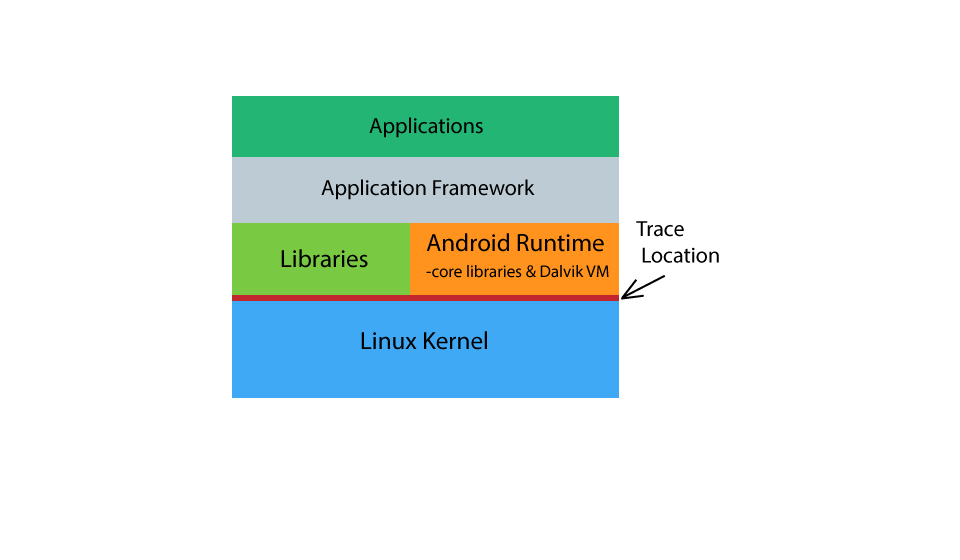
\includegraphics[width=90mm]{images/environment_graphic.png}
  }
  \caption{The Android environment stack. Trace location marks where we will be intercepting system calls}
  
 \end{figure}

With this in mind we set out find a way of measuring mobile battery usage at very low level
(software wise). We decided a good approach would involve monitoring activity at the system 
call level using a tool like strace. Ideally, we want to profile a variety of system calls 
based on how much battery is used while they are running. We intend to establish a baseline 
battery consumption level so we know how much battery is used by just the OS. Then, using 
simple programs that repeatedly make the same system call X times, we can determine how much 
battery was used as a result of initiating a particular system call X times.

Once system calls have been profiled, we can proceed to the last phase of the analysis. Our 
goal is to identify the system calls initiated by the Dalvik VM as a result of running an 
individual app. By identifying the types of system calls, as well as the number of calls made 
to an individual system call, we will be able to predict the app's impact on the battery based 
on what we learned about battery usage for individual system calls. While this approach may not 
be the most accurate, we believe it is the broadest approach that will allow us to profile any 
application regardless of the author or the nature of the software's license.

\section{Milestones}
\uline{Milestone 1}\\
To begin the project we want to: 
\begin{itemize}
  \item Compile small list of most used system calls by profiling a handful of popular android applications
  \item Compile simple C programs (on linux/android) that runs the list most used system calls
  \item Collect data on battery usage as a result of running the C programs on the device
\end{itemize}

\noindent
\uline{Milestone 2}\\
After we have collected data on system calls, we will:
\begin{itemize}
  \item Search for the most suitable tracing platform and trace system calls on various applications 
  \item Identify and analyze the types of system calls and the number of each call initiated by individual applications
\end{itemize}

\noindent
\uline{Milestone 3}\\
With all this data in hand, the last step is to:
\begin{itemize}
  \item Organize the data collected
  \item Attempt identification of patterns and relationships between system calls and battery usage by statistically analyzing the data
  \item Use established relationships to predict battery usage of a novel application
\end{itemize}

\bibliographystyle{cs65f12}
\bibliography{cs65f12}

\end{document}
